\documentclass[12pt,a4paper]{article}

% Packages
\usepackage[utf8]{inputenc}
\usepackage[T1]{fontenc}
\usepackage{lmodern}
\usepackage[margin=1in]{geometry}
\usepackage{graphicx}
\usepackage{hyperref}
\usepackage{xcolor}
\usepackage{listings}
\usepackage{booktabs}
\usepackage{tabularx}
\usepackage{longtable}
\usepackage{enumitem}
\usepackage{fancyhdr}
\usepackage{titlesec}
\usepackage{float}
\usepackage{tikz}
\usepackage{amssymb}
\usepackage{pifont}
\usepackage{multicol}
\usepackage{tcolorbox}
\usetikzlibrary{shapes.geometric, arrows, positioning, fit, backgrounds, calc}

% Custom checkmarks and crosses
\newcommand{\cmark}{\ding{51}}
\newcommand{\xmark}{\ding{55}}

% Colors
\definecolor{primary}{HTML}{3B82F6}
\definecolor{secondary}{HTML}{10B981}
\definecolor{accent}{HTML}{F59E0B}
\definecolor{danger}{HTML}{EF4444}
\definecolor{codebg}{HTML}{F3F4F6}
\definecolor{codetext}{HTML}{1F2937}
\definecolor{progressfill}{HTML}{22C55E}
\definecolor{progressbg}{HTML}{E5E7EB}

% Hyperref setup
\hypersetup{
    colorlinks=true,
    linkcolor=primary,
    filecolor=primary,
    urlcolor=primary,
    citecolor=primary,
    pdftitle={Auctioneer - Project Status & Roadmap},
    pdfauthor={Auctioneer Development Team},
}

% Code listing style
\lstdefinestyle{codestyle}{
    backgroundcolor=\color{codebg},
    basicstyle=\ttfamily\small\color{codetext},
    breakatwhitespace=false,
    breaklines=true,
    captionpos=b,
    keepspaces=true,
    showspaces=false,
    showstringspaces=false,
    showtabs=false,
    tabsize=2,
    frame=single,
    rulecolor=\color{gray!30},
    xleftmargin=0.5cm,
    xrightmargin=0.5cm,
}
\lstset{style=codestyle}

% Header/Footer
\pagestyle{fancy}
\fancyhf{}
\fancyhead[L]{Auctioneer - Project Status}
\fancyhead[R]{January 2026}
\fancyfoot[C]{\thepage}
\renewcommand{\headrulewidth}{0.4pt}
\renewcommand{\footrulewidth}{0.4pt}

% Title formatting
\titleformat{\section}
{\normalfont\Large\bfseries\color{primary}}{\thesection}{1em}{}
\titleformat{\subsection}
{\normalfont\large\bfseries\color{secondary}}{\thesubsection}{1em}{}
\titleformat{\subsubsection}
{\normalfont\normalsize\bfseries\color{accent}}{\thesubsubsection}{1em}{}

% Custom tcolorbox styles
\tcbuselibrary{skins,breakable}

\newtcolorbox{infobox}[1][]{
    colback=primary!5,
    colframe=primary,
    fonttitle=\bfseries,
    title=#1,
    breakable
}

\newtcolorbox{warningbox}[1][]{
    colback=accent!5,
    colframe=accent,
    fonttitle=\bfseries,
    title=#1,
    breakable
}

\newtcolorbox{dangerbox}[1][]{
    colback=danger!5,
    colframe=danger,
    fonttitle=\bfseries,
    title=#1,
    breakable
}

\newtcolorbox{successbox}[1][]{
    colback=secondary!5,
    colframe=secondary,
    fonttitle=\bfseries,
    title=#1,
    breakable
}

% Document info
\title{
    \vspace{-2cm}
    {\Huge\textbf{\textcolor{primary}{Auctioneer}}}\\[0.3cm]
    {\Large Project Status \& Roadmap}\\[0.5cm]
    \rule{\textwidth}{0.4pt}
}
\author{}
\date{
    \textbf{Last Updated:} January 10, 2026\\
    \textbf{Current Phase:} Development (Iteration 1) $\rightarrow$ Bugfixing\\[0.5cm]
    Version 1.0
}

\begin{document}

% Title page
\maketitle
\thispagestyle{empty}

\vfill
\begin{center}

\begin{tikzpicture}
    % Progress bar background
    \fill[progressbg, rounded corners=3pt] (0,0) rectangle (12,0.6);
    % Progress bar fill (40%)
    \fill[progressfill, rounded corners=3pt] (0,0) rectangle (4.8,0.6);
    % Progress text
    \node at (6,0.3) {\textbf{\textcolor{white}{40\% Complete}}};
\end{tikzpicture}
\end{center}
\vfill

\newpage

% Table of Contents
\tableofcontents
\newpage

% ============================================================================
% SECTION 1: SYSTEM OVERVIEW
% ============================================================================
\section{System Overview}

\textbf{Auctioneer} is a real-time auction platform that enables users to:

\begin{itemize}
    \item \textbf{Sell items} through timed auctions with live bidding
    \item \textbf{Direct selling} for fixed-price transactions
    \item \textbf{Barter} items with other users
    \item \textbf{Chat} in real-time during auctions
    \item \textbf{Track} bids and receive notifications
\end{itemize}

\subsection{Core User Flows}

\begin{table}[H]
\centering
\begin{tabularx}{\textwidth}{|l|X|}
\hline
\textbf{Role} & \textbf{Capabilities} \\
\hline
\textbf{Buyer} & Browse auctions, place bids, chat, buy directly, propose barters \\
\hline
\textbf{Seller} & Create listings (auction/direct/barter), manage items, view analytics \\
\hline
\textbf{Guest} & Browse public auctions (view only) \\
\hline
\end{tabularx}
\caption{User Roles and Capabilities}
\end{table}

% ============================================================================
% SECTION 2: TECH STACK
% ============================================================================
\section{Tech Stack}

\subsection{Frontend}

\begin{table}[H]
\centering
\begin{tabularx}{\textwidth}{|l|X|}
\hline
\textbf{Technology} & \textbf{Purpose} \\
\hline
Next.js 15 & React framework with App Router \\
\hline
TypeScript & Type safety \\
\hline
Tailwind CSS & Styling \\
\hline
Zustand & State management (auth store) \\
\hline
Socket.IO Client & Real-time communication \\
\hline
Lucide React & Icons \\
\hline
\end{tabularx}
\caption{Frontend Technology Stack}
\end{table}

\subsection{Backend}

\begin{table}[H]
\centering
\begin{tabularx}{\textwidth}{|l|X|}
\hline
\textbf{Technology} & \textbf{Purpose} \\
\hline
Express.js & REST API server \\
\hline
TypeScript & Type safety \\
\hline
Socket.IO & WebSocket server for real-time features \\
\hline
JWT & Authentication tokens \\
\hline
bcrypt & Password hashing \\
\hline
\end{tabularx}
\caption{Backend Technology Stack}
\end{table}

\subsection{Database \& DevOps}

\begin{table}[H]
\centering
\begin{tabularx}{\textwidth}{|l|X|}
\hline
\textbf{Technology} & \textbf{Purpose} \\
\hline
PostgreSQL & Primary database \\
\hline
Prisma ORM & Database access \& migrations \\
\hline
Turborepo & Monorepo management \\
\hline
pnpm & Package management \\
\hline
\end{tabularx}
\caption{Database and DevOps Stack}
\end{table}

% ============================================================================
% SECTION 3: ARCHITECTURE
% ============================================================================
\section{Architecture}

\subsection{System Architecture}

\begin{figure}[H]
\centering
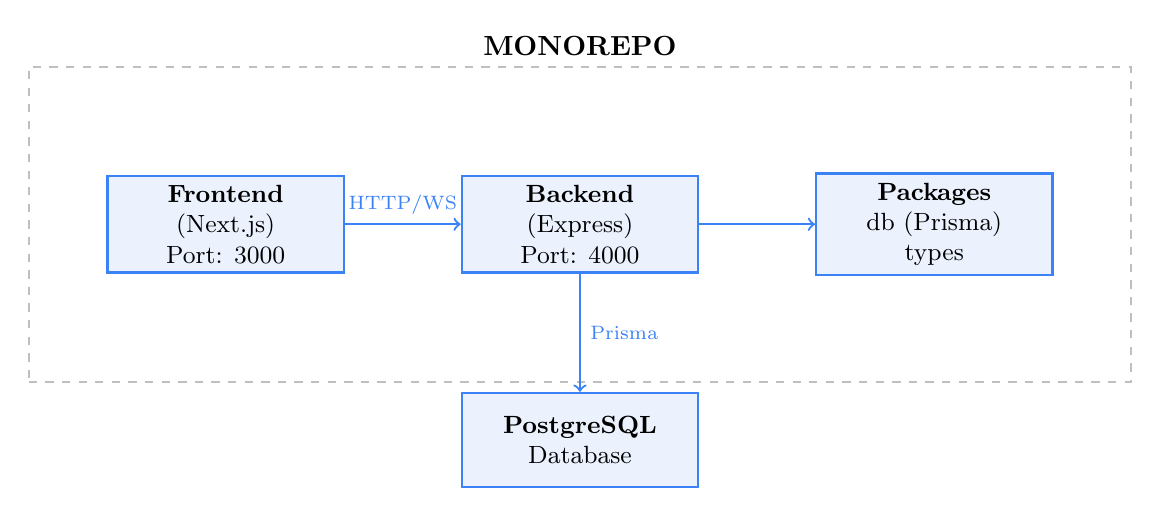
\begin{tikzpicture}[
    node distance=0.8cm,
    box/.style={rectangle, draw=primary, fill=primary!10, thick, minimum width=3cm, minimum height=1.2cm, align=center, font=\small},
    container/.style={rectangle, draw=gray!50, dashed, thick, inner sep=0.4cm},
]

% Monorepo container
\node[container, minimum width=14cm, minimum height=4cm] (monorepo) at (0,0) {};
\node[above] at (monorepo.north) {\textbf{MONOREPO}};

% Frontend
\node[box] (frontend) at (-4.5,0) {\textbf{Frontend}\\(Next.js)\\Port: 3000};

% Backend
\node[box] (backend) at (0,0) {\textbf{Backend}\\(Express)\\Port: 4000};

% Packages
\node[box] (packages) at (4.5,0) {\textbf{Packages}\\db (Prisma)\\types};

% Database
\node[box, below=1.5cm of backend] (database) {\textbf{PostgreSQL}\\Database};

% Arrows
\draw[->, thick, primary] (frontend) -- node[above, font=\scriptsize] {HTTP/WS} (backend);
\draw[->, thick, primary] (backend) -- (packages);
\draw[->, thick, primary] (backend) -- node[right, font=\scriptsize] {Prisma} (database);

\end{tikzpicture}
\caption{High-Level System Architecture}
\end{figure}

\subsection{Data Models}

\begin{figure}[H]
\centering
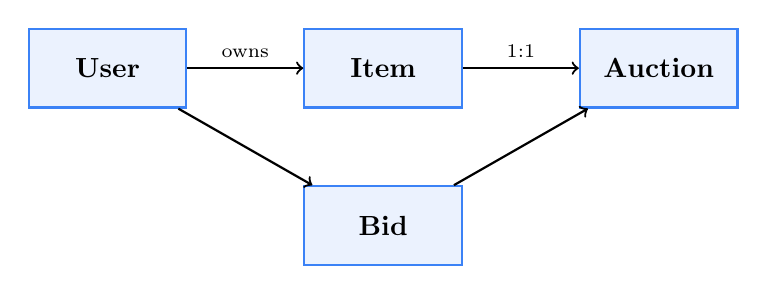
\begin{tikzpicture}[
    entity/.style={rectangle, draw=primary, fill=primary!10, thick, minimum width=2cm, minimum height=1cm, align=center},
]

\node[entity] (user) at (0,0) {\textbf{User}};
\node[entity] (item) at (3.5,0) {\textbf{Item}};
\node[entity] (auction) at (7,0) {\textbf{Auction}};
\node[entity] (bid) at (3.5,-2) {\textbf{Bid}};

\draw[->, thick] (user) -- node[above, font=\scriptsize] {owns} (item);
\draw[->, thick] (item) -- node[above, font=\scriptsize] {1:1} (auction);
\draw[->, thick] (user) -- (bid);
\draw[->, thick] (bid) -- (auction);

\end{tikzpicture}
\caption{Entity Relationship Diagram}
\end{figure}

% ============================================================================
% SECTION 4: FEATURE STATUS
% ============================================================================
\section{Feature Status}

\subsection{Completed Features}

\begin{successbox}[\cmark~Completed]
\begin{tabularx}{\textwidth}{|l|X|}
\hline
\textbf{Feature} & \textbf{Notes} \\
\hline
User Authentication & Login, Register, JWT tokens \\
\hline
Auction CRUD (Backend) & Create, Read, Update, Delete \\
\hline
Item Management (Backend) & Create items linked to auctions \\
\hline
Seller Dashboard & View/manage auctions \\
\hline
Delete Auction & With confirmation modal \\
\hline
Responsive Layouts & Seller dashboard, auction pages \\
\hline
\end{tabularx}
\end{successbox}

\subsection{In Progress}

\begin{warningbox}[In Progress]
\begin{tabularx}{\textwidth}{|l|l|X|}
\hline
\textbf{Feature} & \textbf{Priority} & \textbf{Notes} \\
\hline
Auction Frontend & \textbf{HIGH} & Auction pages need completion \\
\hline
Live Bidding & \textbf{HIGH} & Backend done, frontend in progress \\
\hline
Auction Chat & \textbf{HIGH} & Backend done, frontend in progress \\
\hline
Image Management & \textbf{HIGH} & No image database yet \\
\hline
Edit Auction Modal & \textbf{HIGH} & Image handling incomplete \\
\hline
Bugfixes & \textbf{HIGH} & See Known Issues section \\
\hline
Notifications & \textbf{HIGH} & Not yet implemented \\
\hline
Design Consistency & \textbf{MEDIUM} & Need design system audit \\
\hline
\end{tabularx}
\end{warningbox}

\subsection{Not Started}

\begin{infobox}[Pending Features]
\begin{tabularx}{\textwidth}{|l|l|l|X|}
\hline
\textbf{Feature} & \textbf{Priority} & \textbf{Complexity} & \textbf{Notes} \\
\hline
Direct Selling CRUDL & HIGH & Medium & Item type in schema \\
\hline
Barter System CRUDL & HIGH & High & Needs proposal flow \\
\hline
Home Recommendations & MEDIUM & Medium & Algorithm TBD \\
\hline
Data Population & MEDIUM & Low & Seed script needed \\
\hline
Bidding System Review & HIGH & Medium & Race conditions \\
\hline
Buying Flow & HIGH & Medium & Checkout integration \\
\hline
Bartering Flow & HIGH & High & Negotiation UI \\
\hline
\end{tabularx}
\end{infobox}

% ============================================================================
% SECTION 5: KNOWN ISSUES
% ============================================================================
\section{Known Issues}

\subsection{Critical Issues}

\begin{dangerbox}[Critical - Immediate Action Required]
\begin{tabularx}{\textwidth}{|X|l|X|}
\hline
\textbf{Issue} & \textbf{Location} & \textbf{Impact} \\
\hline
Broken \texttt{findUnique} query & AuthServices.ts:35 & Registration may fail \\
\hline
Hardcoded JWT fallback secret & websocket/index.ts & Security vulnerability \\
\hline
Bidding race condition & auctionWebSocket.ts & Duplicate winning bids \\
\hline
Chat messages in memory & chatWebSocket.ts & Data loss on restart \\
\hline
CORS wide open & backend/index.ts & Security vulnerability \\
\hline
\end{tabularx}
\end{dangerbox}

\subsection{Medium Issues}

\begin{warningbox}[Medium Priority]
\begin{tabularx}{\textwidth}{|X|l|X|}
\hline
\textbf{Issue} & \textbf{Location} & \textbf{Impact} \\
\hline
User enumeration & AuthController.ts & Security concern \\
\hline
Password exposed in responses & AuctionServices.ts & Privacy leak \\
\hline
No input validation & Multiple controllers & Data integrity \\
\hline
Username not unique in DB & schema.prisma & Duplicate usernames \\
\hline
No cascade deletes & schema.prisma & Orphaned data \\
\hline
Socket reconnection issues & SocketContext.tsx & UX issue \\
\hline
Hardcoded localhost URLs & Multiple files & Production issues \\
\hline
\end{tabularx}
\end{warningbox}

\subsection{Minor Issues}

\begin{infobox}[Minor - Low Priority]
\begin{tabularx}{\textwidth}{|X|l|X|}
\hline
\textbf{Issue} & \textbf{Location} & \textbf{Impact} \\
\hline
Unused imports & Multiple files & Code cleanliness \\
\hline
Deprecated \texttt{.substr()} & chatWebSocket.ts & Future compatibility \\
\hline
No bid confirmation dialog & LiveBidding.tsx & Accidental bids \\
\hline
\end{tabularx}
\end{infobox}

% ============================================================================
% SECTION 6: PIPELINE PROGRESS
% ============================================================================
\section{Pipeline Progress}

\subsection{Overall Progress}

\begin{figure}[H]
\centering
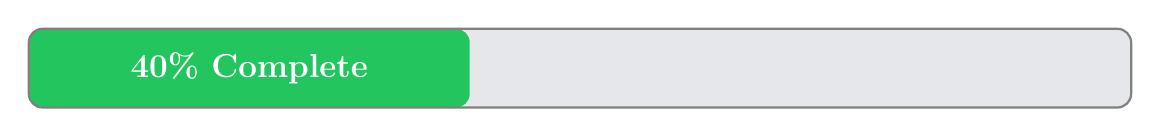
\begin{tikzpicture}
    % Progress bar background
    \fill[progressbg, rounded corners=5pt] (0,0) rectangle (14,1);
    % Progress bar fill (40%)
    \fill[progressfill, rounded corners=5pt] (0,0) rectangle (5.6,1);
    % Percentage text
    \node[white, font=\bfseries\large] at (2.8,0.5) {40\% Complete};
    % Border
    \draw[gray, thick, rounded corners=5pt] (0,0) rectangle (14,1);
\end{tikzpicture}
\caption{Phase 1 Pipeline Progress}
\end{figure}

\subsection{Phase Breakdown}

\begin{table}[H]
\centering
\begin{tabularx}{\textwidth}{|l|c|X|}
\hline
\textbf{Phase} & \textbf{Status} & \textbf{Progress} \\
\hline
Development (Iteration 1) & \textcolor{accent}{$\circlearrowright$} & \textbf{IN PROGRESS} ($\sim$70\%) \\
\hline
Staging & \textcolor{accent}{$\circlearrowright$} & IN PROGRESS \\
\hline
QA & $\square$ & NOT STARTED \\
\hline
Bugfixing & \textcolor{accent}{$\circlearrowright$} & IN PROGRESS ($\sim$40\%) \\
\hline
Testing & $\square$ & NOT STARTED \\
\hline
Development (Iteration 2) & $\square$ & OPTIONAL \\
\hline
Initial Deployment & $\square$ & NOT STARTED \\
\hline
\end{tabularx}
\caption{Pipeline Phase Status}
\end{table}

\subsection{Milestone Timeline}

\begin{table}[H]
\centering
\begin{tabularx}{\textwidth}{|l|l|X|}
\hline
\textbf{Milestone} & \textbf{Status} & \textbf{Notes} \\
\hline
Backend API & \textcolor{secondary}{\cmark~Complete} & Done \\
\hline
Seller Dashboard & \textcolor{secondary}{\cmark~Complete} & Done \\
\hline
Auction Frontend & \textcolor{accent}{In Progress} & $\sim$50\% \\
\hline
Live Bidding (FE) & \textcolor{accent}{In Progress} & $\sim$30\% \\
\hline
Chat (Frontend) & \textcolor{accent}{In Progress} & $\sim$30\% \\
\hline
Image Storage & $\square$~Pending & No DB yet \\
\hline
Critical Bugfixes & \textcolor{accent}{In Progress} & $\sim$40\% \\
\hline
Direct Selling & $\square$~Pending & -- \\
\hline
Barter System & $\square$~Pending & -- \\
\hline
Investor Demo Ready & $\square$~Pending & Target: After QA \\
\hline
\end{tabularx}
\caption{Milestone Timeline}
\end{table}

% ============================================================================
% SECTION 7: NEXT STEPS
% ============================================================================
\section{Next Steps}

\subsection{Immediate (This Sprint)}

\subsubsection{1. Fix Critical Security Issues}

\begin{lstlisting}[language=bash]
# Priority order:
1. AuthServices.ts - Fix broken findUnique query
2. websocket/index.ts - Remove hardcoded JWT fallback
3. backend/index.ts - Configure CORS properly
4. Add input sanitization for chat (XSS prevention)
\end{lstlisting}

\subsubsection{2. Fix Bidding Race Condition}

\begin{itemize}
    \item Implement Prisma transactions for atomic bid placement
    \item Add minimum bid increment validation
    \item Consider anti-sniping protection
\end{itemize}

\subsubsection{3. Environment Configuration}

\begin{itemize}
    \item Create \texttt{.env.example} files
    \item Move all hardcoded URLs to environment variables
    \item Document required environment variables
\end{itemize}

\subsection{Short Term (Next 2 Sprints)}

\subsubsection{4. Complete Notifications System}

\begin{itemize}
    \item Define notification types (outbid, auction ending, won, etc.)
    \item Create notifications table in database
    \item Implement real-time push via WebSocket
    \item Add notification UI component
\end{itemize}

\subsubsection{5. Direct Selling Implementation}

\begin{itemize}
    \item Backend API endpoints for direct sales
    \item Frontend listing creation (type: DIRECT)
    \item Buy Now button and checkout flow
    \item Order/transaction tracking
    \item Seller confirmation flow
\end{itemize}

\subsubsection{6. Persist Chat Messages}

\begin{itemize}
    \item Add \texttt{Message} model to Prisma schema
    \item Migrate from in-memory to database storage
    \item Add message history loading on room join
\end{itemize}

\subsection{Medium Term (Before Investor Demo)}

\subsubsection{7. Barter System}

\begin{itemize}
    \item Barter proposal data model
    \item Proposal creation UI
    \item Accept/Reject/Counter flow
    \item Barter history tracking
    \item Notification integration
\end{itemize}

\subsubsection{8. Home Page \& Recommendations}

\begin{itemize}
    \item Define recommendation algorithm (trending, ending soon, category-based)
    \item Create seed script for demo data
    \item Implement recommendation API endpoints
    \item Build home page components
\end{itemize}

\subsubsection{9. Design System Audit}

\begin{itemize}
    \item Document color palette, typography, spacing
    \item Create shared component library
    \item Ensure dark/light mode consistency
    \item Mobile responsiveness review
\end{itemize}

\subsection{Pre-Deployment}

\subsubsection{10. Testing Suite}

\begin{itemize}
    \item Unit tests for critical services
    \item Integration tests for API endpoints
    \item E2E tests for core user flows
\end{itemize}

\subsubsection{11. Performance \& Security Hardening}

\begin{itemize}
    \item Add rate limiting
    \item Implement Helmet.js
    \item Database query optimization (indexes)
    \item Load testing
\end{itemize}

% ============================================================================
% SECTION 8: PRE-DEPLOYMENT CHECKLIST
% ============================================================================
\section{Pre-Deployment Checklist}

\subsection{Security}

\begin{itemize}[label=$\square$]
    \item Remove all hardcoded secrets
    \item Configure CORS for production domain
    \item Add rate limiting
    \item Add Helmet.js security headers
    \item Implement token blacklist for logout
    \item Add input validation/sanitization
    \item Security audit of auth flow
\end{itemize}

\subsection{Database}

\begin{itemize}[label=$\square$]
    \item Add \texttt{@unique} to username
    \item Add cascade deletes
    \item Add performance indexes
    \item Create production migration strategy
    \item Seed script for initial data
\end{itemize}

\subsection{Infrastructure}

\begin{itemize}[label=$\square$]
    \item Environment variables documented
    \item Production database setup
    \item SSL certificates
    \item Domain configuration
    \item CI/CD pipeline
    \item Monitoring \& logging
    \item Backup strategy
\end{itemize}

\subsection{Code Quality}

\begin{itemize}[label=$\square$]
    \item Remove console.logs
    \item Remove unused imports
    \item Fix TypeScript \texttt{any} types
    \item Code review completed
    \item Documentation updated
\end{itemize}

\subsection{Testing}

\begin{itemize}[label=$\square$]
    \item Critical path E2E tests pass
    \item Load testing completed
    \item Cross-browser testing
    \item Mobile testing
\end{itemize}

% ============================================================================
% SECTION 9: INVESTOR DEMO NOTES
% ============================================================================
\section{Notes for Investor Demo}

\subsection{Demo Flow Suggestion}

\begin{enumerate}
    \item \textbf{Landing Page} -- Show platform value proposition
    \item \textbf{Browse Auctions} -- Demonstrate item discovery
    \item \textbf{Live Auction} -- Show real-time bidding (use 2 browsers)
    \item \textbf{Seller Dashboard} -- Demonstrate seller experience
    \item \textbf{Create Auction} -- Quick listing creation
    \item \textbf{Chat Feature} -- Real-time communication
\end{enumerate}

\subsection{Recommended Demo Data}

\begin{itemize}
    \item 10-15 sample auctions across categories
    \item 3-5 active auctions with bids
    \item 2-3 auctions ending within demo timeframe
    \item Sample user accounts (buyer, seller)
\end{itemize}

\subsection{Talking Points}

\begin{infobox}[Key Messages]
\begin{itemize}
    \item \textbf{Real-time bidding technology} -- Instant updates, no page refresh
    \item \textbf{Multi-platform marketplace} -- Auction, direct sale, and barter options
    \item \textbf{Scalable architecture} -- Built for growth with modern stack
    \item \textbf{Growth potential} -- Expanding to additional transaction types
\end{itemize}
\end{infobox}

% ============================================================================
% SECTION 10: DOCUMENTATION LINKS
% ============================================================================
\section{Documentation Links}

\begin{table}[H]
\centering
\begin{tabularx}{\textwidth}{|l|X|}
\hline
\textbf{Document} & \textbf{Description} \\
\hline
SYSTEM\_DESIGN.md & Detailed system architecture and data models \\
\hline
WEBSOCKET\_GUIDE.md & WebSocket implementation and event reference \\
\hline
README.md & Quick start guide and project overview \\
\hline
Auctioneer\_Documentation.tex & Full technical documentation (this series) \\
\hline
\end{tabularx}
\caption{Related Documentation}
\end{table}

\vfill

\begin{center}
\rule{0.5\textwidth}{0.4pt}\\[0.5cm]
\textit{This document should be updated as development progresses.}
\end{center}

\end{document}
